\section{System Architecture}

\todo{Physical Architectural View}

As previously mentioned, there are many layers of abstraction in the program before one actually reaches the hardware level of the sensors. In this section, we will describe these layers, going from the high-level programming of the model, e.g. the architecture described in figure \ref{fig:softwareArchitecture}, down to the hardware specifics of the sensors themselves. 

The intent is, of course, that these software abstractions will not affect our model implementation, aside from the fact that we have to include some libraries to facilitate sensor communication (for instance "ecrobot\_interface.h" and similar). See figure \ref{fig:abstractionLayers} for the system architecture and its layers of abstraction. The dark blue object "Components" consists of all the software inside the components planned in the previous section \ref{fig:softwareArchitecture}. 

\todo{mention that it is a layer diagram, going from top, high-level to hardware sensors and actuators}
\todo{More corrections from 8/11-2017}
\begin{figure}[H]
    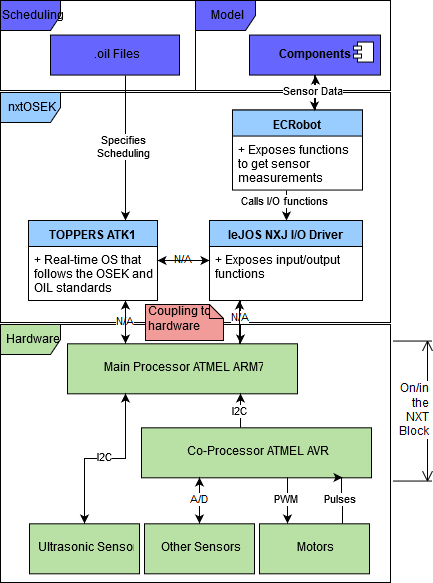
\includegraphics[width=\textwidth]{Images/Design/abstractionLayerDiagram.png}
    \caption{Layer diagram of the system architecture of the product, going from high-level programming down to low-level hardware specifics.
    \todo[inline]{From supervisor: These arrows mean different things than other arrows inside the box, so they must be drawn somehow differently.
I am reading these as layers in OSI model, e.g.
http://www.flickriver.com/photos/phploveme/2911722148/}}
    \label{fig:abstractionLayers}
\end{figure}

The note "Coupling to hardware" and the "N/A" edges exists because those are implementation details inside nxtOSEK, which we do not really have access to\todo{From supervisor: Just treat it as a different abstraction layer. It is not realy an API, nor protocol, but something that "runs on top".}. In the hardware frame, the edges signify communication protocols such as PWM (pulse width modulation, as described in section \ref{analysisMotors}). 
